\documentclass{ximera}  


\input{../preamble.tex}



 
\title{Waves on Transmission Lines} 
\author{Milica Markovic} 
\outcome{Apply phasor transformation to a time-domain equation to obtain frequency-domain equation.}
\begin{document}  
\begin{abstract}  

\end{abstract}  
\maketitle    






Any wire, cable or line that guides energy from one point to another
is a transmission line. Whenever you make a circuit on a breadboard,
every wire you attach makes  a transmission line with the ground wire. Whether we see the propagation (transmission line) effects on the
line depends on the line length. 
At lower frequencies or very short line lengths we do not
see any difference between the signal's phase at the generator and at the load,
whereas at higher frequencies we do.








\section{Types of transmission lines}

\begin{enumerate}
\item Coaxial Cable, Figure \ref{fig:qm/Coax}
\item Microstrip, Figure \ref{fig:qm/MStrip}
\item Stripline, Figure \ref{fig:qm/Strp}
\item Coplanar Waveguide, Figure \ref{fig:qm/CPW}
\item Two-wire line, Figure \ref{fig:qm/TwoWL}
\item Parallel Plate Waveguide, Figure \ref{fig:qm/PPW}
\item Rectangular Waveguide, Figure \ref{fig:qm/RecWG}
\item Optical fiber, Figure \ref{fig:qm/OF}
\end{enumerate}




\begin{figure}[ht!]
\begin{center}
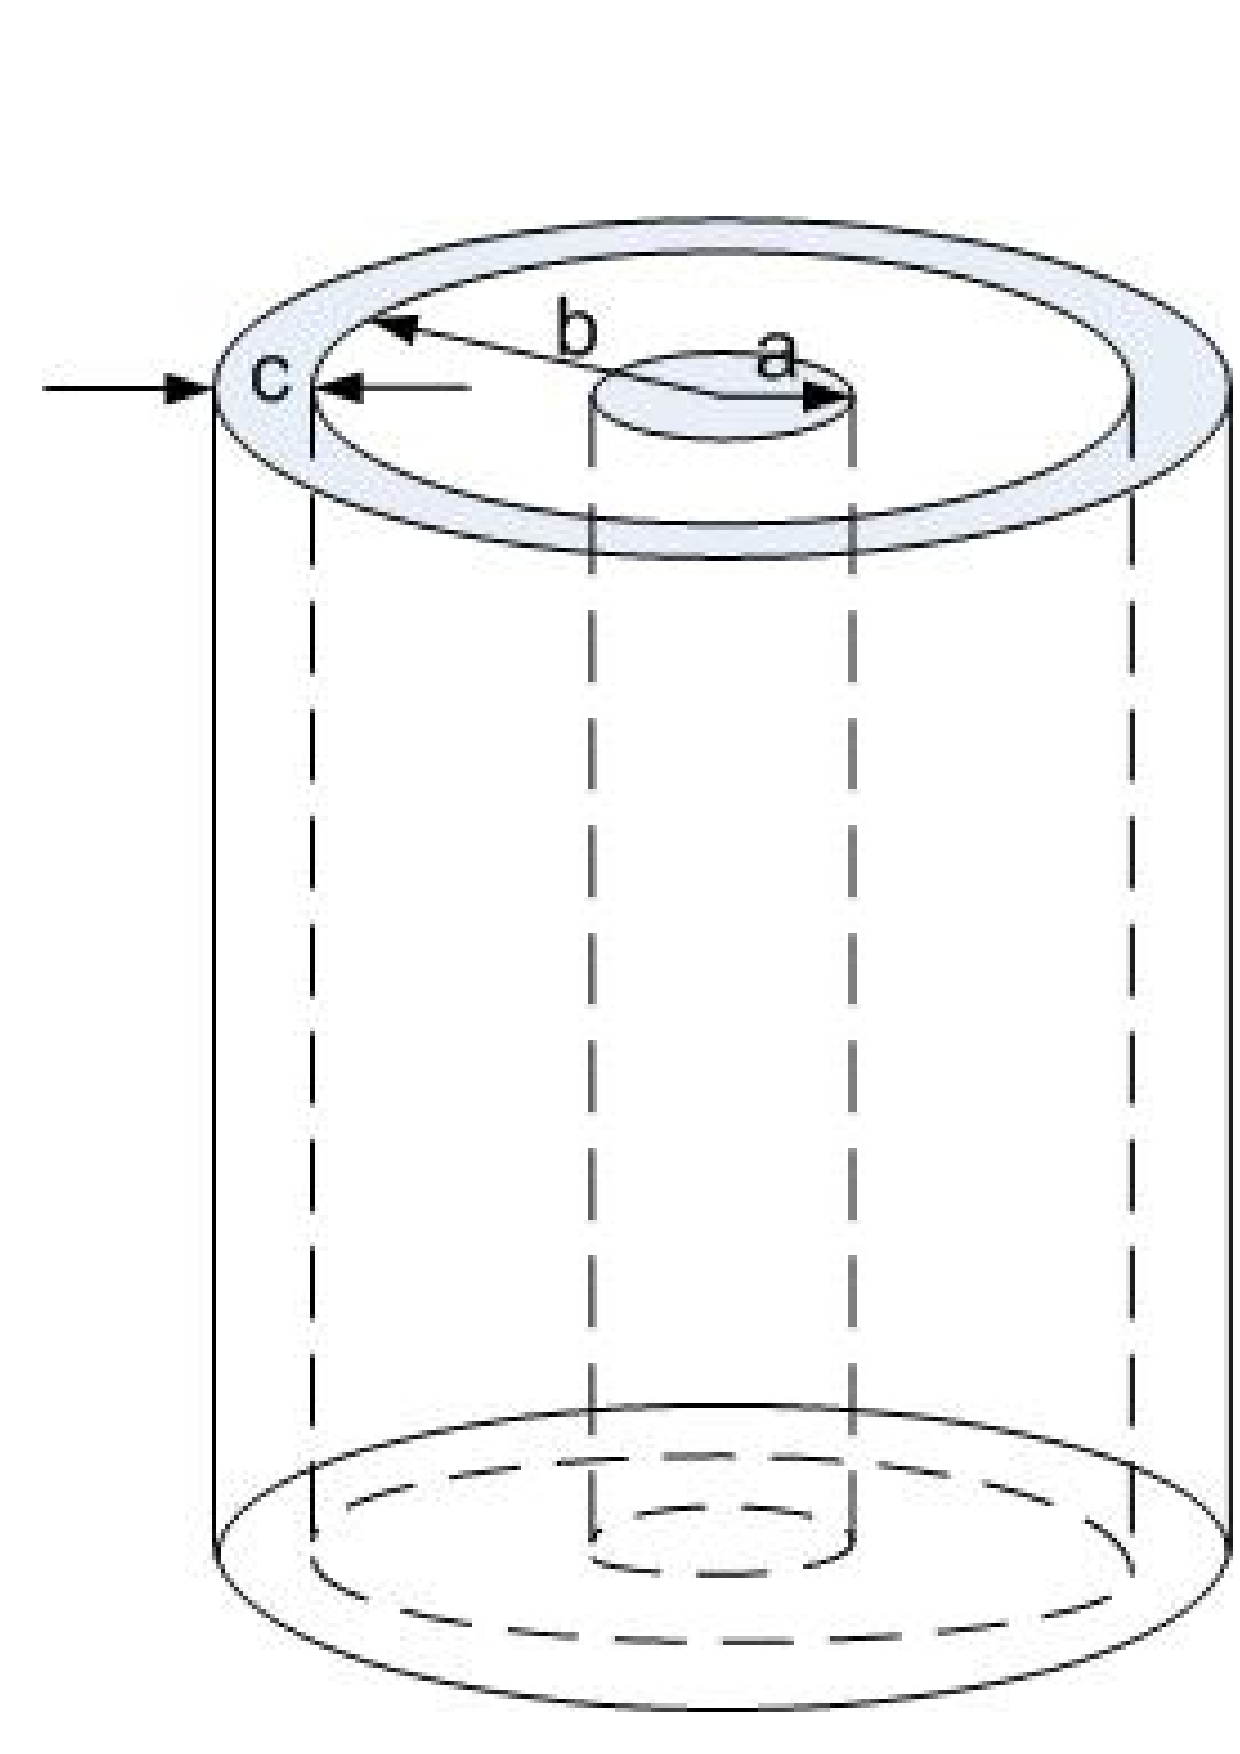
\includegraphics[scale=0.4]{../jpg/coax.jpg}
\caption{\label{fig:qm/Coax} Coaxial Cable}
\end{center}
\end{figure}


\begin{figure}[ht!]
\begin{center}
\includegraphics[scale=0.4]{../jpg/microstrip.jpg}
\caption{\label{fig:qm/MStrip} Microstrip}
\end{center}
\end{figure}

\begin{figure}[ht!]
\begin{center}
\includegraphics[scale=0.4]{../jpg/stripline.jpg}
\caption{\label{fig:qm/Strp} Stripline.}
\end{center}
\end{figure}

\begin{figure}[ht!]
\begin{center}
\includegraphics[scale=0.4]{../jpg/cpw.jpg}
\caption{\label{fig:qm/CPW} Coplanar Waveguide.}
\end{center}
\end{figure}

\begin{figure}[ht!]
\begin{center}
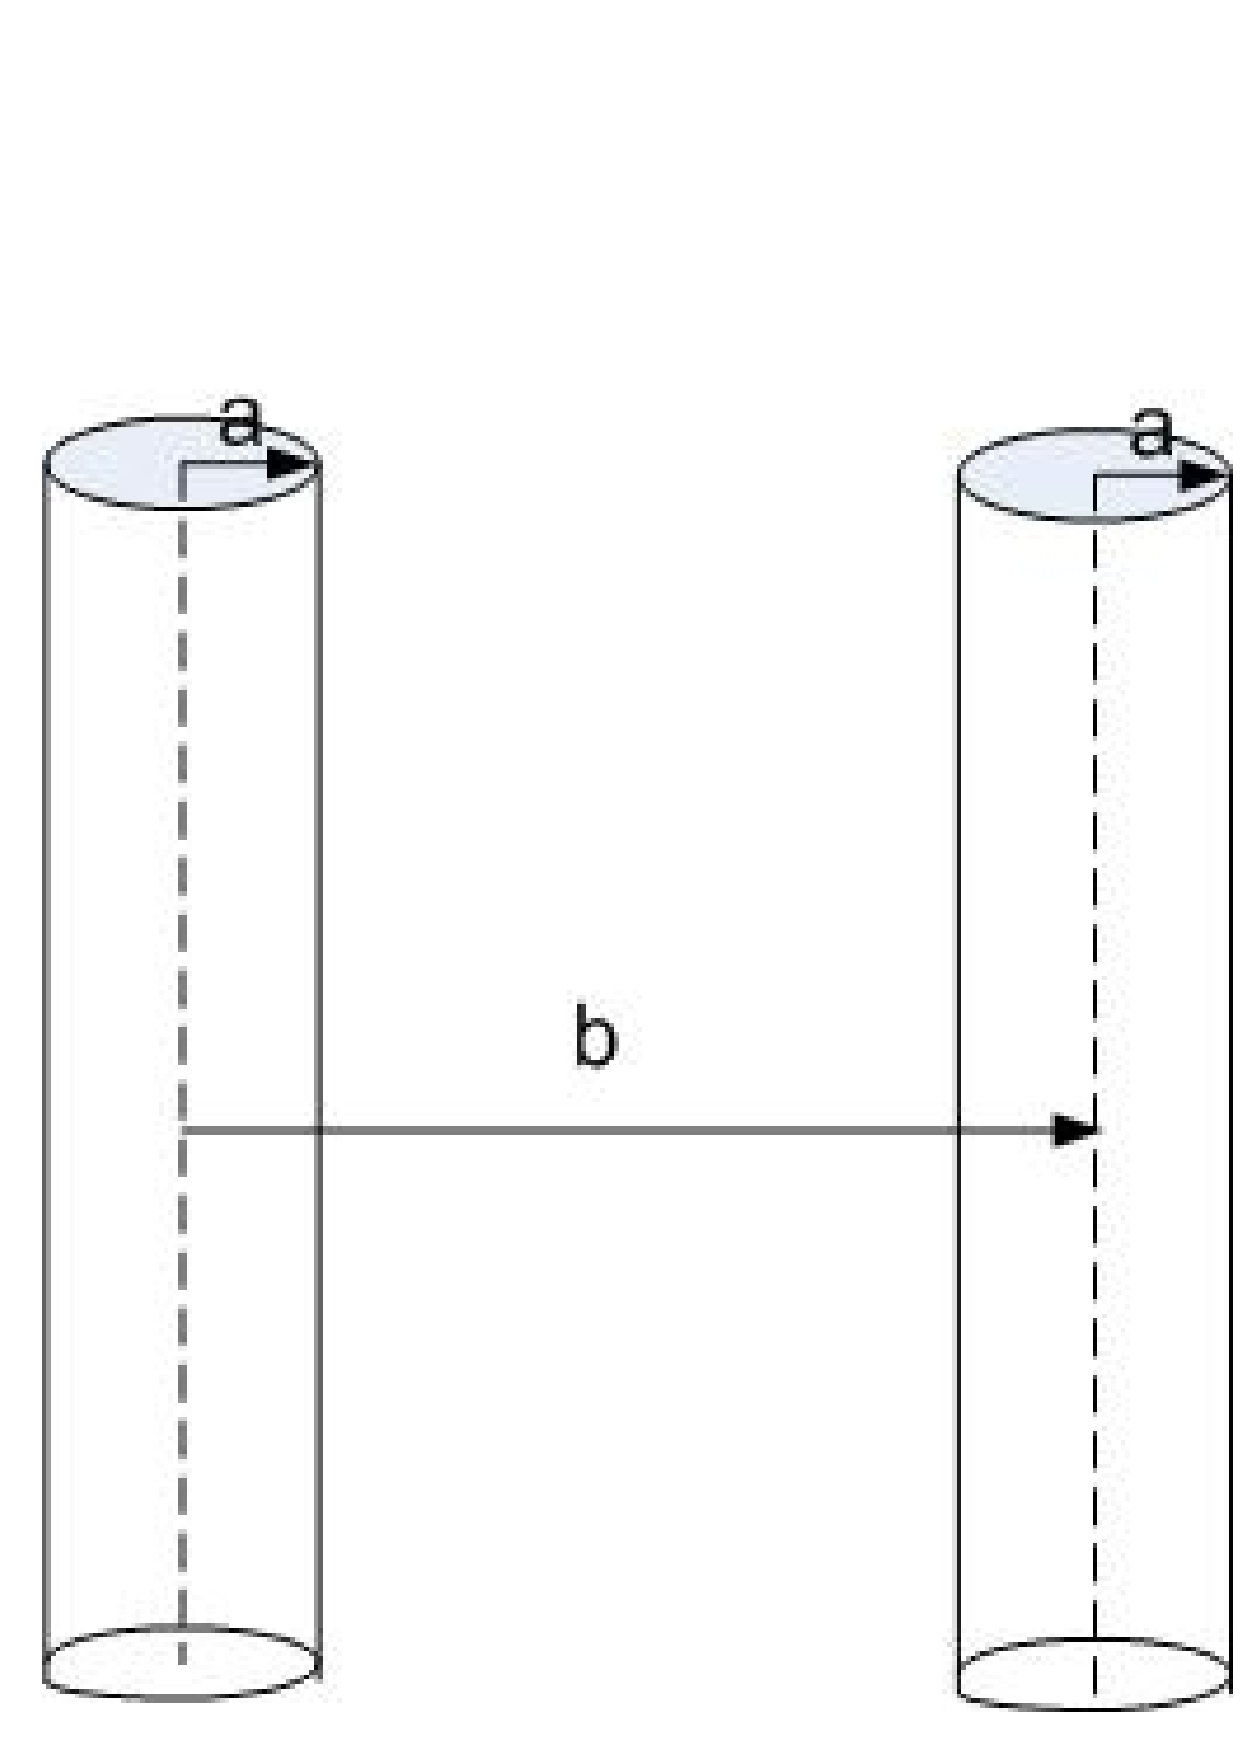
\includegraphics[scale=0.4]{../jpg/twowireline.jpg}
\caption{\label{fig:qm/TwoWL} Two-wire line.}
\end{center}
\end{figure}

\begin{figure}[ht!]
\begin{center}
\includegraphics[scale=0.4]{../jpg/ppw.jpg}
\caption{\label{fig:qm/PPW} Parallel-Plate Waveguide.}
\end{center}
\end{figure}

\begin{figure}[ht!]
\begin{center}
\includegraphics[scale=0.4]{../jpg/rectwg.jpg}
\caption{\label{fig:qm/RecWG} Rectangular Waveguide.}
\end{center}
\end{figure}

\begin{figure}[ht!]
\begin{center}
\includegraphics[scale=0.4]{../jpg/fiber.jpg}
\caption{\label{fig:qm/OF} Optical Fiber.}
\end{center}
\end{figure}


\section{What are Transmission Line Effects?}

Figure \ref{timedelaysig} shows a step voltage at the generator and the load of a circuit in Figure \ref{elcric}. The voltage needs T sec to appear at the load, once the switch closes. Figure \ref{delayedsig} shows the step signal as it traveles on the transmission line at different time steps t=0, t=T/4, t=T/2 and t=T.
How much time it takes for this signal to go from AA' end to BB' end? 
Since electromagnetic waves propagate with the constant speed, the speed of light, time that  the signal needs to go from the generator to  the load  depends  on the length of the transmission line $ l$.  $T=\frac{l}{c}$, where $c=3\, 10^8$. If the signal at the generator AA' is


\begin{figure}[htbp]
\begin{center}
\includegraphics[scale=0.5]{../jpg/timedelayedsignal.jpg}  
%\strut\psfig{figure=generaltransmissionlinecircuit.ps,width=3cm}
\end{center}
\caption{Voltage as a function of time at the generator side z=0 (top) and the load side z=l (bottom) of the transmission line in Figure \ref{elcric}, if the switch closes at t=0 the voltage arrives at t=l/c=T at the load. These graphs can be obtained by observing the voltage on an oscilloscope at the load and at the generator side.}
\label{timedelaysig}  \end{figure}



\begin{figure}[htbp]
\begin{center}
\includegraphics[scale=0.5]{../jpg/timedelayedsignaltl.jpg}
%\strut\psfig{figure=generaltransmissionlinecircuit.ps,width=3cm} \\
\end{center}
\caption{Voltage along the transmission line in Figure \ref{elcric}, for four different time intervals t=0, switch closes, t=T/4, t=T/2 and t=T. It is assumed that the length of the transmission line is equal to l=T/c.}
\label{delayedsig}
\end{figure}




\begin{figure}[htbp]
\begin{center}
\includegraphics[scale=0.5]{../jpg/generaltransmissionlinecircuit1.jpg}
%\strut\psfig{figure=generaltransmissionlinecircuit.ps,width=3cm} \\
\end{center}
\caption{Electronic Circuit with an emphasis on cables that connect the generator and the load.}
\label{elcric}
\end{figure}



\begin{eqnarray}
v_{AA^`}(t)=A cos(\omega t)
\end{eqnarray}

Then at the other end the transmission line the signal is


\begin{eqnarray}
v_{BB^`}(t)=v_{AA^`}(t-T) \\
v_{BB^`}(t)=v_{AA^`}(t-\frac{l}{c}) \\
v_{BB^`}(t)=A cos(\omega (t - \frac{l}{c}))  \\
v_{BB^`}(t)=A cos(\omega t - \omega \frac{l}{c}) \\
v_{BB^`}(t)=A cos(\omega t -  \frac{\omega }{c} l) 
\end{eqnarray}

Since we know that angular frequency is  $\omega = 2 \pi f$


\begin{eqnarray}
v_{BB^`}(t)=A cos(\omega t -  \frac{ 2 \pi f }{c} l)
\end{eqnarray}

The quantity $\frac{c}{f}$ is called the wavelength $\lambda$. 

\begin{eqnarray}
v_{BB^`}(t)=A \, cos(\omega t -  \frac{ 2 \pi }{\lambda} l) \label{tllength1}
\end{eqnarray}

The quantity $ \frac{ 2 \pi }{\lambda} $ is the propagation constant $\beta$


Finally the expression for the voltage at BB end is


\begin{eqnarray}
v_{BB^`}(t)=A \, cos(\omega t - \beta l) \\
v_{BB^`}(t)=A \, cos(\omega t - \Psi)
\end{eqnarray}

We see that at BB' the signal will experience a phase shift.
We will derive this equation  again later from the Telegrapher's
equations.
Now let's see how the length of the line $l$ affects the voltage at the
end BB'. Look at Equation \ref{tllength1}.
The signal will experience a phase shift of $2\pi \frac{l}{\lambda}$. If this phase shift is small, there will not be much difference between
the phase of the signal at the generator and at the load. This means that we don't have to use transmission line theory to account for the effects of the line.
If the phase shift is significant, then we do have to use the transmission line theory. Let's look at some numbers in the  following example.

\begin{enumerate}
\item If $\frac{l}{\lambda} < 0.01$ then the angle $2 \pi
\frac{l}{\lambda}$ is of the order of 0.0314 rad or about 2$^0$. In this case, the
phase is obviosly something that we don't have to worry about. When
the length of the transmission line is much smaller than $\lambda$, $l<<\frac{\lambda}{100}$
the wave propagation on the line can be ingnored.
\item If  $\frac{l}{\lambda} > 0.01$, say  $\frac{l}{\lambda} =0.1$,
then the phase is 20$^0$, which is a significant phase shift. In this
case it may be necessary to account fro transmission line effects.
\end{enumerate}



\section{Propagation modes on a transmission line}

Coax, two wire line, microstrip etc can be approximated as TEM up to
the 30-40\,GHz (unshielded), up to 140\,GHz shielded.




\begin{enumerate}
\item Transversal Electro-Magnetic Field (TEM). Electric (E), and Magnetic (M) fields are entirely transversal to the direction of
propagation
\item Transversal Electric field (TE), Transversal Magnetic Field (TM),  M or E field is in the direction of propagation
\end{enumerate}

Transmission lines that we are discussing  here cary TEM fields.


\section{ Wave equation on a transmission line}\label{telegrapher}

In this section we will derive the expression for voltage and current
along a transmission line. This expression will have two variables, time $t$ and space $z$. 
So far we have only seen voltages and currents  as a function of time.  This is because all circuit elements seen so far were lumped elements. In distributed systems
we want to derive the equations for voltage and current for the case when the transmission
line is longer then the fraction of a wavelength.  To make sure that we
don't encounter any  transmission line effects to start with, we can
look at the piece of a transmission line that is much smaller then
the fraction of a wavelength. In other words we cut the transmission
line into small pieces to make sure there are no transmission line
effects, as the pieces are shorter then the fraction of a wavelength. We then represent each piece with
an equivalent circuit as shown in Figure \ref{lineeqc} (a). 
To derive expressions for current and voltage on transmission line we will use the following five-step plan

\begin{enumerate}
\item Look at an infinitesimal length of a transmission line $\Delta z$.  

\item Represent that piece with an equivalent circuit. 

\item Write KCL, KVL for the piece in the time domain (we get
differential equations)

\item Apply phasors (equations become linear)

\item Solve the linear system of equations to get the expression for
the voltage and current on the transmission line as a function of $z$.

\end{enumerate}


Let's follow the plan now. Look at a small piece of a transmission line and represented it with an equivalent circuit. What is
modeled by the circuit elements?



\begin{figure}[htbp]
\begin{center}
\includegraphics[scale=0.3]{../jpg/Coaxtl.jpg}
\caption{Coaxial cable is cut in short pieces.}
\label{lineeqcPieces}
\end{center}
\end{figure}

\begin{figure}[htbp]
\begin{center}
\includegraphics[scale=0.3]{../jpg/Equivalent_Circuit_of_Transmission_Line.jpg}
\caption{Equivalent circuit of a section of transmission line.}
\label{lineeqcOnePiece}
\end{center}
\end{figure}

\begin{figure}[htbp]
\begin{center}
\includegraphics[scale=0.4]{../jpg/tlmadeupofcircuits.jpg}
\end{center}
\caption{Equivalent circuit of transmission line.}
\label{lineeqc}
\end{figure}



Write  KVL and KCL equations for the circuit above.

KVL
\begin{eqnarray}
-v(z,t) + R \Delta z  i(z,t) + L \Delta z \frac{\partial
 i(z,t)}{\partial t} + v(z+ \Delta z,t) = 0 \nonumber
\end{eqnarray}

KCL

\begin{eqnarray}
i(z,t)=i(z+\Delta z)+ i_{CG}(z+\Delta z,t) \nonumber   \\
i(z,t)=i(z+\Delta z)+ G \Delta z v(z+\Delta z,t)+C\Delta z
\frac{\partial v(z+\Delta z,t)}{\partial t} \nonumber
\end{eqnarray}


Rearrange the KCL and KVL Equations \ref{te1kvl1}, \ref{te1kc11} and divide them with
$\Delta z$.  Equations \ref{te2kvl1}, \ref{te1kc21}.
let $\Delta z \to 0$ and recognize the definition of the
derivative Equations, \ref{te2kvl111}, \ref{te1kc211}.

KVL
\begin{eqnarray}
-( v(z+ \Delta z ,t)- v(z,t))=R \Delta z i(z,t)+L \Delta z
 \frac{\partial i(z,t)}{\partial t} \label{te1kvl1}  \\ 
 -\frac{ v(z+ \Delta z ,t)- v(z,t)}{\Delta z}=R i(z,t)+L 
 \frac{\partial i(z,t)}{\partial t}  \label{te2kvl1} \\
\lim_{\Delta z \to 0} \{ -\frac{ v(z+ \Delta z ,t)- v(z,t)}{\Delta z}\}=  \lim_{\Delta z \to 0} \{   R i(z,t)+L 
 \frac{\partial i(z,t)}{\partial t} \} \label{te2kvl111} \\
-\frac{v(z,t) }{\partial z}=R i(z,t)+L 
 \frac{\partial i(z,t)}{\partial t} \label{te3kvl1}
\end{eqnarray}

KCL

\begin{eqnarray}
-( i(z+ \Delta z ,t)- i(z,t))= G \Delta z v(z+\Delta z,t)+C\Delta z
\frac{\partial v(z+\Delta z,t)}{\partial t} \label{te1kc11} \\
-\frac{ i(z+ \Delta z ,t)- i(z,t)}{\Delta z}= G v(z+\Delta z,t)+C
\frac{\partial v(z+\Delta z,t)}{\partial t} \label{te1kc21} \\
\lim_{\Delta z \to 0} \{-\frac{ i(z+ \Delta z ,t)- i(z,t)}{\Delta z} \}= \lim_{\Delta z \to 0} \{ G v(z+\Delta z,t)+C
\frac{\partial v(z+\Delta z,t)}{\partial t} \} \label{te1kc211} \\
-\frac{i(z,t) }{\partial z}= G v(z+\Delta z,t)+C
\frac{\partial v(z+\Delta z,t)}{\partial t} \label{te1kc31}
\end{eqnarray}



We just derived Telegrapher's equations in time-domain:



\begin{eqnarray}
-\frac{v(z,t) }{\partial z}=R i(z,t)+L 
 \frac{\partial i(z,t)}{\partial t} \nonumber  \\ \nonumber
-\frac{i(z,t) }{\partial z}= G v(z+\Delta z,t)+C
\frac{\partial v(z+\Delta z,t)}{\partial t} 
\end{eqnarray}


Telegrapher's equations are two differential equations with two unknowns, $i(z, t)$, $v(z, t)$. It is not
impossible to solve them, however we would prefer to have linear 
equations. We then express time-domain variables as phasors.

\begin{eqnarray}
v(z,t)=Re\{ \tilde{V}(z) e^{j \omega t} \} \nonumber \\
i(z,t)=Re\{ \tilde{I}(z) e^{j \omega t} \} \nonumber
\end{eqnarray}

Where $\tilde{V}(z),\tilde{I}(z) $ are the voltage and current anywhere on the line, and depend on the position on the line $z$. And we get the Telegrapher's equations in phasor form


\begin{eqnarray}
-\frac{\partial \tilde{V}(z)}{\partial z} = (R+j\omega L) \tilde{I}(z) \label{te11}\\
-\frac{\partial \tilde{I}(z)}{\partial z} = (G+j\omega C) \tilde{V}(z) \label{te121}
\end{eqnarray}



Two equations, two unknowns. To solve these equations, we first
take a derivative of  both equations with respect to  z. 

\begin{eqnarray}
-\frac{\partial^2 \tilde{V}(z)}{\partial z^2}=  (R+j\omega L) \frac{\partial
 \tilde{I}(z)}{\partial z}  \label{teleg3} \\
-\frac{\partial^2 \tilde{I}(z)}{\partial z^2}=  (G+j\omega C) \frac{\partial
 \tilde{V}(z)}{\partial z} \label{teleg4}
\end{eqnarray}

Rearange the previous equations:



\begin{eqnarray}
- \frac{1}{ (R+j\omega L)} \frac{\partial \tilde{I}(z)}{\partial z}= \frac{\partial^2
  \tilde{V}(z)}{\partial z^2} \label{te51} \\
-\frac{1}{ (G+j\omega C)} \frac{\partial \tilde{V}(z)}{\partial z}= \frac{\partial^2
  \tilde{I}(z)}{\partial z^2} \label{te61}
\end{eqnarray}

Substitute  Eq.\ref{te51} into  Eq.\ref{te121}
and Eq.\ref{te61} into Eq.\ref{te11} and we get

\begin{eqnarray}
-\frac{\partial^2 \tilde{V}(z)}{\partial z^2}=(G+j\omega C)(R+j\omega L) \tilde{V}(z) \label{teleg1} \\
-\frac{\partial^2 \tilde{I}(z)}{\partial z^2}= (G+j\omega C)  (R+j\omega L) \label{teleg2}
\tilde{I}(z) 
\end{eqnarray}

Or if we rearrange


\begin{eqnarray}
\frac{\partial^2 \tilde{V}(z)}{\partial z^2} -(G+j\omega C)(R+j\omega L)
 \tilde{V}(z)=0  \label{we11} \\ 
\frac{\partial^2 I(z)}{\partial z^2}- (G+j\omega C)  (R+j\omega L)
I(z)=0 \label{we21}
\end{eqnarray}

The above Eq.\ref{we11} and Eq.\ref{we21} are called the wave equation, and  they represent
current and voltage wave on a transmission line. $\gamma=(G+j\omega
C)(R+j\omega L)$ is the complex propagation constant. This constant
has a real and an imaginary part.

\begin{eqnarray}
\gamma= \alpha + j \beta \nonumber
\end{eqnarray}

where $\alpha$ is the attenuation constant and $\beta$ is the phase
constant.

\begin{eqnarray}
\alpha=Re\{ \sqrt{(G+j\omega C)  (R+j\omega L)  }  \} \nonumber \\ \nonumber
\beta = Im\{ \sqrt{(G+j\omega C)  (R+j\omega L)  }  \}
\end{eqnarray}

The general solution of the second order differential equations with constant coefficients
Equations \ref{we11} - \ref{we21}   is:

\begin{eqnarray}
\tilde{\tilde{V}(z)}=\tilde{V_0}^+ e^{-\gamma z} + \tilde{V_0}^- e^{\gamma z} \nonumber \\ \nonumber
\tilde{I(z)}=\tilde{I_0}^+ e^{-\gamma z} + \tilde{I_0}^- e^{\gamma z}
\end{eqnarray}

In this equation $\tilde{V_0}^+$ and $\tilde{V_0}^-$ are the {\bf
phasors} of forward and
reflected voltage waves at the load (where z=0), and $\tilde{I_0}^+$ and $\tilde{I_0}^-$ are the phasors of forward and
reflected  current wave at the load (where z=0).These voltages and currents are also phasors and have a constant magnitude and phase in a specific circuit, for example $\tilde{V_0}^+=|\tilde{V_0}^+| e^\Phi=4e^{25^0}$, and $\tilde{I_0}^+=|\tilde{I_0}^+| e^\Phi=5e^{-40^0}$.
The time domain expression for the current and voltage on the
transmission line we can get by multiplying the phasor of the voltage and current with $e^{j \omega t}$ and taking the real part of it.

\begin{eqnarray}
v(t)=Re\{ (\tilde{V}_0^+  e^{(-\alpha - j \beta) z} + \tilde{V}_0^- e^{(\alpha + j
 \beta) z})e^{j \omega t} \}  \nonumber \\ 
v(t)=|\tilde{V}_0^+| e^{ - \alpha z} \cos(\omega t - \beta z + \angle \tilde{V}_0^+)+
|\tilde{V}_0^-|e^{\alpha z} \cos(\omega t + \beta z + \angle \tilde{V}_0^-) \label{tdeq}
\end{eqnarray}

We'll look at the Matlab program the next class to see that if the signs of the $\omega t$ and
$\beta z$ are the same the wave moves in the forward $+z$
direction. If the signs of $\omega t$ and $\beta z$ are opposite, the
wave moves in the $-z$ direction.



\section{Visualization of Lossless Forward and Reflected Voltage Waves}

We will show next that if  the signs of the $\omega t$ and
$\beta z$ are the same, as in Equation \ref{bck1}, the wave moves in the forward $+z$
direction. If the signs of $\omega t$ and $\beta z$ are opposite, as in Equation \ref{fwd1}, the
wave moves in the $-z$ direction. In order to see this, we will visualize Equations \ref{fwd1} and \ref{bck1} using Matlab code below.

\begin{eqnarray}
v_f(t)=|\tilde{V}_0^+| e^{ - \alpha z} \cos(\omega t - \beta z + \angle \tilde{V}_0^+) \label{fwd1} \\
v_r(t)= |\tilde{V}_0^-|e^{\alpha z} \cos(\omega t + \beta z + \angle \tilde{V}_0^-) \label{bck1}
\end{eqnarray}


Figure \ref{fwrdref}  shows forward and reflected waves on a transmission line. On x-axis is the spatial coordinate $z$ from the generator to the load, where the transmission line is connected,  and on y-axis is   the magnitude of the voltage on the line.   The red line on both graphs is the voltage signal at a time  .1 ns. We would obtain  Figure \ref{fwrdref} if we had a camera that can take picture of voltages, and we took the first picture at $t_1=$ .1 ns on the entire transmission line.  The blue dotted line on both graphs is the same signal .1 ns later,  at time $t_2=$.2  ns.  We see that the signal has moved to the right in the time of 1 ns, or from the generator to the load.  On the bottom graph we see that at a time .1 ns, the red line represents the  reflected signal.  Dashed blue line shows the signal  at a time .2 ns. We see  that  the signal has moved to the left, or  from the load to the generator. 


\begin{figure}[ht!]
\begin{center}
\includegraphics[scale=0.5]{../jpg/frwrdwave_01.jpg}
\caption{\label{fwrdref} Forward (top) and reflected (bottom) waves on a transmission line.}
\end{center}
\end{figure}


\begin{verbatim}
clear all
clc
f = 10^9;
w = 2*pi*f
c=3*10^8;
beta=2*pi*f/c;
lambda=c/f;
t1=0.1*10^(-9)
t2=0.2*10^(-9)
x=0:lambda/20:2*lambda;

y1=sin(w*t1 - beta.*x);
y2=sin(w*t2 - beta.*x);
y3=sin(w*t1 + beta.*x);
y4=sin(w*t2 + beta.*x);

subplot (2,1,1),

    plot(x,y1,'r'),...
            hold on
    plot(x,y2,'--b'),...
    hold off
subplot (2,1,2),

    plot(x,y3,'r')
        hold on
    plot(x,y4,'--b')
    hold off
\end{verbatim}

Using matlab code above, repeat the visualization of signals  in the previous section for a lossy transmission line. Assume that $\alpha=0.1$\,Np, and all other variables are the same as in the previous section. How do the voltages compare in the lossy and lossless cases?

\section{Relating forward and backward current and voltage waves on
the transmission line}


In equations \ref{eq4}-\ref{eq5} $\tilde{V}_0^+$ and $\tilde{V}_0^-$ are the phasors of forward and
reflected going voltage waves, and $\tilde{I}_0^+$ and $\tilde{I}_0^-$ are the phasors of forward and
reflected  current waves. In this section, we will see how the phasors of forward and reflected voltage and
current waves are related to transmission line impedance.


\begin{eqnarray}
\tilde{V}(z)=\tilde{V}_0^+ e^{-\gamma z} + \tilde{V}_0^- e^{\gamma z}\label{eq4} \\
I(z)=\tilde{I}_0^+ e^{-\gamma z} + \tilde{I}_0^- e^{\gamma z}\label{eq5}
\end{eqnarray}




When substitute the voltage wave equation into Telegrapher's  Equations
\ref{te11}. The equation is repeated here  Eq.\ref{te12new}-\ref{te12new1}.




\begin{eqnarray}
-\frac{\partial \tilde{V}(z)}{\partial z} = (R+j\omega L) I(z) \label{te12new} \\
\gamma \tilde{V}_0^+ e^{-\gamma z} - \gamma \tilde{V}_0^- e^{\gamma z} = (R+ j \omega
L) I(z) \label{te12new1}
\end{eqnarray}

We now rearrange Eq.\ref{te12new1}

\begin{eqnarray}
I(z)=\frac{\gamma}{R+j\omega L} ( \tilde{V}_0^+ exp^{-\gamma z} + \tilde{V}_0^-
 exp^{\gamma z})  \nonumber  \\
I(z)=\frac{\gamma \tilde{V}_0^+}{R+ j \omega L} e^{-\gamma z} - \frac{\gamma \tilde{V}_0^-}{R+ j \omega L} e^{\gamma z} \label{eq3}
\end{eqnarray}

Now we compare Eq.\ref{eq3} with the Eq.\ref{eq5}. In order for two transcendental equations to be equal, the coefficients next to exponential terms have to be the same.

\begin{eqnarray}
\tilde{I}_0^+=\frac{\gamma \tilde{V}_0^+}{R+ j \omega L} \nonumber  \\
\tilde{I}_0^-= - \frac{\gamma \tilde{V}_0^-}{R+ j \omega L} \nonumber
\end{eqnarray}

We can define the characteristic impedance of a transmission line as
the ratio of the voltage to current amplitude of the forward going
wave.


\begin{eqnarray}
Z_0=\frac{\tilde{V}_0^+}{ \tilde{I}_0^+} \nonumber   \\ \nonumber
Z_0=\frac{R+j\omega L}{\gamma} \nonumber   \\ \nonumber
Z_0=\sqrt{\frac{R+j\omega L}{G+ j\omega C}}
\end{eqnarray}


\section{Lossless transmission line}


In many practical applications $R\to 0$ \footnote{metal resistance is
low}and $G \to 0$\footnote{dielectric conductance is low}. This is a
lossless transmission line.

In this case the transmission line parameters are
\begin{itemize}
\item Propagation constant


\begin{eqnarray}
\gamma =\sqrt{(R+j\omega L)(G+ j\omega C)} \nonumber   \\ \nonumber
\gamma= \sqrt{j \omega L j \omega C} \\ \nonumber
\gamma = j \omega \sqrt{L C} = j \beta
\end{eqnarray}

\item Transmission line impedance 

\begin{eqnarray}
Z_0=\sqrt{\frac{R+j\omega L}{G+ j\omega C}} \nonumber  \\ \nonumber
Z_0=\sqrt{\frac{j\omega L}{ j\omega C}} \\ \nonumber
Z_0=\sqrt{\frac{L}{C}}
\end{eqnarray}

\item Wave velocity

\begin{eqnarray}
v=\frac{\omega}{\beta}  \nonumber \\ \nonumber
v=\frac{\omega}{\omega \sqrt{LC}} \\ \nonumber
v=\frac{1}{\sqrt{LC}}
\end{eqnarray}


\item Wavelength


\begin{eqnarray}
\lambda = \frac{2 \pi}{\beta}  \nonumber \\ \nonumber
\lambda = \frac{2 \pi}{ \omega \sqrt{LC}} \\ \nonumber
\lambda =\frac{2 \pi}{\sqrt{\epsilon_0 \mu_0 \epsilon_r} } \\ \nonumber
\lambda = \frac{c}{f \sqrt{\epsilon_r}} \\ \nonumber
\lambda = \frac{\lambda_0}{\sqrt{\epsilon_r}} \nonumber
\end{eqnarray}
\end{itemize}






\section{What does it mean when we say a medium is lossy or lossless?}
In a lossless medium electromagnetic wave power is not turning into heat, there is no loss of amplitude. In lossy medium electromagnetic wave is heating up the medium, therefore its power is decreasing as $e^{-\alpha x}$.




\begin{center}
\begin{tabular}{|c|c|} \hline
medium     & attenuation constant $\alpha$ [dB/km]     \\  \hline       
coax        & 60                                 \\ \hline
 waveguide  & 2  \\ \hline          
fiber-optic &  0.5  \\ \hline
\end{tabular}
\end{center}


In guided wave systems such as transmission lines and waveguides the attenuation of power with distance follows approximately $e^{-2\alpha x}$. The power radiated by an antenna falls off as $1/r^{2}$.

\section{Low-Loss Transmission Line}




In some practical applications, losses are small, but not negligible.  $R<< \omega L$ \footnote{metal resistance is
lower than the inductive impedance}and $G <<  \omega C$\footnote{dielectric conductance is lower than the capacitive impedance}. 

In this case the transmission line parameters are
\begin{itemize}
\item Propagation constant

We can re-write the propagation constant as shown below. 
In somel applications,  losses are small, but not negligible.  $R<< \omega L$ and $G <<  \omega C$, then
in Equation \ref{lossytl2}, $ RG<< \omega^2 LC$.

\begin{eqnarray}
\gamma =\sqrt{(R+j\omega L)(G+ j\omega C)}   \\ 
\gamma= j\omega \sqrt{ L\, C}\sqrt{1\,-\,j\,\left( \frac{R}{\omega L}+\frac{G}{\omega C} \right)-\frac{R G}{\omega^2  L  C}} \label{lossytl2} \\ 
\gamma\approx j\omega \sqrt{ L\, C}\sqrt{1\,-\,j\,\left( \frac{R}{\omega L}+\frac{G}{\omega C} \right)}\label{lowtleq1}
\end{eqnarray}

Taylor's series for function $\sqrt{1+x}= \sqrt{1\,-\,j\,\left( \frac{R}{\omega L}+\frac{G}{\omega C} \right)}$ in Equation \ref{lowtleq1} is shown in Equations \ref{taylorser1}-\ref{taylorser2}.

\begin{eqnarray}
\sqrt{1+x}=1+\frac{x}{2}-\frac{x^2}{8}+\frac{x^3}{16}-...  \,for\, |x|<1 \label{taylorser1} \\
\gamma \approx  j\omega \sqrt{ L\, C} \sqrt{1\,-\,j\,\left( \frac{R}{\omega L}+\frac{G}{\omega C} \right)}= j\omega \sqrt{ L\, C}\left(1-\frac{j}{2} \left(  \frac{R}{\omega L}+\frac{G}{\omega C} \right)\right) \label{taylorser2}
\end{eqnarray}


The real and imaginary part of the propagation constant  $\gamma$ are:

\begin{eqnarray}
\alpha=  \frac{   \omega \sqrt{ L\, C}  }{2} \left(  \frac{R}{\omega L}+\frac{G}{\omega C} \right)  \\
\beta=     \omega \sqrt{ L\, C}
\end{eqnarray}


We see that the phase constant $\beta$ is the same as in the lossless case, and the attenuation constant $\alpha$ is frequency independent. This means that all frequencies of a modulated signal are attenuated the same amount, and there is no dispersion on the line. When the phase constant is a linear function of frequency, $\beta=const \, \omega$, then the phase velocity is a constant $v_p=\frac{\omega}{\beta}=\frac{1}{const}$, and the group velocity is also a constant, and equal to the phase velocity. In this case, all frequencies of the modulated signal are propagated with the same speed, and there is no distortion of the signal. This is the case only when the losses in the transmission line are small. 

We usually represent phase and group velocity on $\omega-\beta$ diagrams, shown in Figure \ref{omegabeta1}. At a frequency $\omega_1$, the ratio of $\frac{\omega}{\beta}$ gives the phase velocity (graphically, this is the slope of the red line on the graph), whereas the slope of the $\omega-\beta$ curve (blue line on the graph) gives the group velocity at this frequency. These diagrams are useful, as they show how phase constant $\beta$ varies with frequency, and it also shows how phase and group velocities vary with frequency. We can see that in this case, both group and phase velocity for this line are positive quantities, which is a representation of what is called a forward wave. In a forward wave, both signal and the energy propagate in the forward direction. Backward waves are waves where the signal propagates forward, however energy propagates backwards. In backward waves, phase and group velocities have opposite signs.  

When the phase constant is a linear function of frequency, then, phase velocity and group velocity are equal, and do not depend on frequency. Both velocities are equal to the slope of the line in Figure \ref{omegabeta2}.

\begin{figure}[htbp]
\begin{center}
\includegraphics[scale=0.6]{../jpg/omegabeta1.jpg}
\caption{Omega-Beta diagrams, Phase constant $\beta$ is a {\bf nonlinear} function of frequency.}\label{omegabeta1}
\end{center}
\end{figure}


\begin{figure}[htbp]
\begin{center}
\includegraphics[scale=0.6]{../jpg/omegabeta2.jpg}
\caption{Omega-Beta diagrams, Phase constant $\beta$ is a {\bf linear} function of frequency.}\label{omegabeta2}
\end{center}
\end{figure}


\end{itemize}




\section{Voltage Reflection Coefficient, Lossless Case}

The equations for the voltage and current on the transmission line we
derived so far are

\begin{eqnarray}
\tilde{V}(z)=\tilde{V}_0^+ e^{-j \beta z} +\tilde{V}_0^- e^{j \beta z} \label{vtl} \\ \label{ctl}
I(z)=\frac{\tilde{V}_0^+}{Z_0} e^{- j \beta z} - \frac{\tilde{V}_0^-}{Z_0} e^{j \beta z}
\end{eqnarray}



\begin{figure}[htbp]
\begin{center}
\includegraphics[scale=0.3]{../jpg/trline.jpg}
%\strut\psfig{figure=trline.ps,width=3cm} \\
\end{center}
\caption{Transmission Line connects generator and the load.}
\label{wind1}
\end{figure}





At $z=0$ the impedance of the load has to be

\begin{eqnarray}
Z_L=\frac{V(0)}{I{0}} \nonumber 
\end{eqnarray}

Substitute the boundary condition in Eq.\ref{vtl}

\begin{eqnarray}
Z_L=Z_0 \frac{\tilde{V}_0^+ + \tilde{V}_0^-}{\tilde{V}_0^+ - \tilde{V}_0^-}
\end{eqnarray}


We can now solve the above equation for $\tilde{V}_0^-$

\begin{eqnarray}
\frac{Z_L}{Z_0} (\tilde{V}_0^+ - \tilde{V}_0^-) = \tilde{V}_0^+ + \tilde{V}_0^- \nonumber \\
(\frac{Z_L}{Z_0}-1)\tilde{V}_0^+ =(\frac{Z_L}{Z_0}+1) \tilde{V}_0^- \nonumber \\
\frac{\tilde{V}_0^-}{\tilde{V}_0^+} = \frac{\frac{Z_L}{Z_0}-1  }{ \frac{Z_L}{Z_0}+1 }
\nonumber \\
\frac{\tilde{V}_0^-}{\tilde{V}_0^+} = \frac{Z_L -Z_0}{Z_L +Z_0}
\end{eqnarray}

The quantity $\frac{\tilde{V}_0^-}{\tilde{V}_0^+}$ is called voltage reflection
coefficient $\Gamma$. It relates the reflected to incident voltage
phasor. Voltage reflection coefficient is in general a complex number,
it has a magnitude and a phase.



\subsubsection{Examples}


 \begin{enumerate}
\item 100\,$\Omega$ transmission line is terminated in a series
connection of a 50\,$\Omega$ resistor and 10\,pF capacitor. The frequency
of operation is 100\,MHz. Find the voltage reflection coefficient.
\item For purely reactive load $Z_L=j X_L$ find the reflection
coefficient.
\end{enumerate}

The end of this lecture is spent in the lab making a Matlab program to
make a movie of a wave moving left and right.


\section{Standing Waves}


In the previous section we introduced the voltage reflection
coefficient that relates the forward to reflected voltage phasor.


\begin{eqnarray}
\Gamma = \frac{\tilde{V}_0^-}{\tilde{V}_0^+} = \frac{Z_L -Z_0}{Z_L +Z_0} \label{reflcoe}
\end{eqnarray}


If we substitute Equation \ref{reflcoe} to Eq.\ref{vtl11} we get for the voltage wave

\begin{eqnarray}
\tilde{V}(z) = \tilde{V}_0^+ e^{-j \beta z} +\tilde{V}_0^- e^{j \beta z} \label{vtl11}\\
\tilde{V}(z) = \tilde{V}_0^+ e^{-j \beta z} + \Gamma  \tilde{V}_0^+ e^{j \beta z} \nonumber
\\
\tilde{V}(z)= \tilde{V}_0^+ (e^{-j \beta z} - \Gamma  e^{j \beta z}  ) \label{vtl01}
\end{eqnarray}

since $\Gamma = |\Gamma| e^{j \Theta_r}$ Eq.\ref{vtl01} becomes


\begin{eqnarray}
\tilde{V}(z)= \tilde{V}_0^+ (e^{-j \beta z} - |\Gamma|  e^{j \beta z + \Theta_r}  ) \label{vtl011}
\end{eqnarray}



and for the current wave



\begin{eqnarray}
I(z) = \frac{\tilde{V}_0^+}{Z_0} e^{-j \beta z} -  \frac{\tilde{V}_0^-}{Z_0} e^{j \beta z} \label{ctl1}\\
I(z) =  \frac{\tilde{V}_0^+}{Z_0}  e^{-j \beta z} + \Gamma \frac{\tilde{V}_0^+}{Z_0}  e^{j \beta z} \nonumber
\\
I(z)=   \frac{\tilde{V}_0^+}{Z_0}  (e^{-j \beta z} - \Gamma  e^{j \beta z}  ) \label{ctl01}
\end{eqnarray}

The voltage and the current waveform on a transmission line are
therefore given by Eqns.\ref{vtl01}, \ref{ctl01}. Now we have two
equations and one unknown $\tilde{V}_0^+$! We will solve these two equations
in Lecture 7. Now let's look at the physical meaning of these
equations.


In Eq.\ref{vtl01}, $\Gamma$ is the voltage reflection coefficient,
$\tilde{V}_0^+$ is the phasor of the forward going wave, $z$ is the axis in
the direction of wave propagation, $\beta$ is the phase
constant\footnote{imaginary part of the complex propagation constant},
$Z_0$ is the impedance of the transmission line\footnote{defined as
the ratio of forward going voltage and current}. $\tilde{V}(z)$ is a complex
number, phasor. We will find the magnitude and phase of the voltage on
the transmission line.




The magnitude of a complex number can be found as $|z|=\sqrt{z
z^*}$.

\begin{eqnarray}
|\tilde{V}(z)|=\sqrt{\tilde{V}(z) \tilde{V}(z)^*} \nonumber  \\
|\tilde{V}(z)|=\sqrt{   \tilde{V}_0^+ (e^{-j \beta z} - |\Gamma|  e^{j \beta z +
 \Theta_r}  )  
   \tilde{V}_0^+ (e^{j \beta z} - |\Gamma|  e^{-(j \beta z + \Theta_r)}     )} \nonumber
\\
|\tilde{V}(z)|= \tilde{V}_0^+ \sqrt{(e^{-j \beta z} - |\Gamma|  e^{j \beta z +
|\Theta_r}  )  
  (e^{j \beta z} - |\Gamma|  e^{-(j \beta z + \Theta_r)}     )}
\nonumber \\
|\tilde{V}(z)|= \tilde{V}_0^+ \sqrt{1+  |\Gamma|  e^{-(2j \beta z +
|\Theta_r)}    + |\Gamma|  e^{j 2 \beta z + \Theta_r} +|\Gamma|^2     )}
\nonumber \\
|\tilde{V}(z)|= \tilde{V}_0^+ \sqrt{1+ |\Gamma|^2 + |\Gamma| ( e^{-(2j \beta z +
 \Theta_r)}   +  e^{(j 2 \beta z + \Theta_r)}     )}
 \nonumber \\
|\tilde{V}(z)|= \tilde{V}_0^+  \sqrt{1+ |\Gamma|^2 + 2 |\Gamma| \cos(2 \beta z +\Theta_r)} \label{sw1} 
\end{eqnarray}

The magnitude of the total voltage on the transmission line is given
by Eq.\ref{sw1}. It seems like a complicated function.

\begin{itemize}
 \item Let's start 
from a simple case when the voltage reflection coefficient on the
tranmission line is $\Gamma=0$ and draw the magnitude of the total
voltage. The magnitude is the green line in Figure \ref{flatline}. To see the movie
of this transmission line go to the class web page under Instructional Videos. Forward voltage is shown in red, reflected voltage in pink,
and the magnitude of the voltage is  green. Magnitude of the voltage is constant everywhere on the transmission line, and so the line
is called flat.




\begin{figure}[htbp]
\begin{center}
\includegraphics[scale=0.3]{../jpg/flatline.jpg}
%\strut\psfig{figure=smithchartreflection.ps,width=3cm} \\
\end{center}
\caption{Flat line.}
\label{flatline}
\end{figure}



\item Let's look at another case,  $\Gamma=0.5$ and $\Theta_r=0$. Equation \ref{swc1}  represents the magnitude of the voltage on the transmission line, and Figure \ref{reflcoeffvid} shows in green how this function looks on a transmission line. This case is shown in Figure \ref{reflcoeffvid}. 

\begin{eqnarray}
|\tilde{V}(z)|=\tilde{V}_0^+ \sqrt{\frac{5}{4}+ cos{2 \beta z} }\label{swc1}
\end{eqnarray}

\begin{figure}[htbp]
\begin{center}
\includegraphics[scale=0.3]{specialcase.jpg}
%\strut\psfig{figure=smithchartreflection.ps,width=3cm} \\
\end{center}
\caption{Voltage on a transmission line with reflection coefficient magnitude 0.5, and zero phase.}
\label{reflcoeffvid}
\end{figure}



The function \ref{swc1} is at it's maximum 
when $cos(2 \beta z)=1$ or $z=\frac{k}{2} \lambda$, and the function
value is $\tilde{V}(z)=1.5\tilde{V}_0^+  $. It is at it's
minimum when  $cos(2 \beta z)=-1$ or $z=\frac{2 k +1}{4} \lambda$
and the function value is $\tilde{V}(z)=0.5 \tilde{V}_0^+$

It is important to mention here that the function that we see looks
like a cosine with an average value of $ \tilde{V}_0^+ $, but {\bf it is not}.
The minimums of the function are sharper then the maximums, so when
the reflection coefficient is at it's maximum of $\Gamma =1$ the
function looks like this:


\begin{figure}[htbp]
\begin{center}
\includegraphics[scale=0.3]{../jpg/shortedline.jpg}
%\strut\psfig{figure=smithchartreflection.ps,width=3cm} \\
\end{center}
\caption{Shorted Transmission Line.}
\label{wind}
\end{figure}



\item General Case. 

In general the voltage maximums will occur when
$cos(2 \beta z)=1$

\begin{eqnarray}
|\tilde{V}(z)_{max}|=\tilde{V}_0^+\sqrt{1+|\Gamma|^2+2 |\Gamma|} \nonumber  \\
|\tilde{V}(z)_{max}| =\tilde{V}_0^+\sqrt{(1+|\Gamma|)^2}  \nonumber \\
|\tilde{V}(z)_{max}| =\tilde{V}_0^+(1+|\Gamma|) 
\end{eqnarray}



In general the voltage minimums will occur when
$cos(2 \beta z)=-1$,



\begin{eqnarray}
|\tilde{V}(z)_{min}|=\tilde{V}_0^+\sqrt{1+|\Gamma|^2-2 |\Gamma|} \nonumber  \\
|\tilde{V}(z)_{min}| =\tilde{V}_0^+\sqrt{(1-|\Gamma|)^2}  \nonumber \\
|\tilde{V}(z)_{min}| =\tilde{V}_0^+ (1-|\Gamma|) 
\end{eqnarray}

The ratio of voltage minimum on the line over the voltage maximum is
called the Voltage Standing Wave Ratio (VSWR) or just Standing Wave
Ratio (SWR).

\begin{eqnarray}
SWR=\frac{\tilde{V}(z)_{max}}{ \tilde{V}(z)_{min}} \nonumber \\
SWR=\frac{1+|\Gamma|}{1-|\Gamma|}
\end{eqnarray}

The voltage maximum position on the line is where
\begin{eqnarray}
cos(2 \beta z)=1 \nonumber \\
2 \beta z + \Theta_r = 2 n \pi \nonumber \\
z =\frac{ 2 n \pi -\Theta_r }{ 2 \beta} \nonumber \\
z=\frac{ 2 n \pi -\Theta_r }{ 4 \pi}
\end{eqnarray}



\end{itemize}




































  Display image.
\begin{image}  
  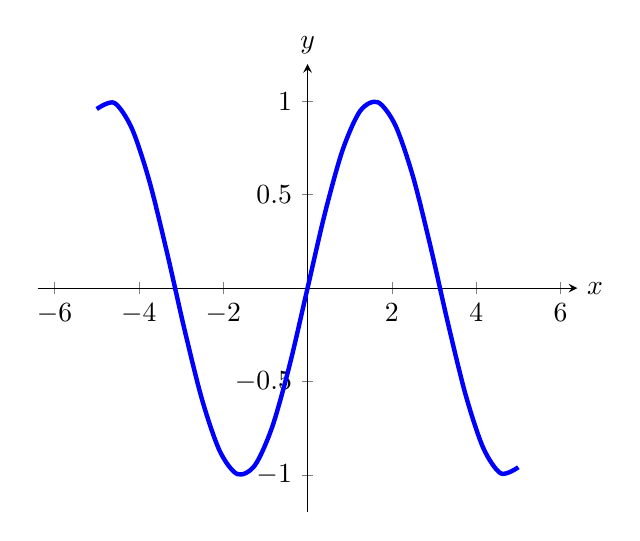
\begin{tikzpicture}  
    \begin{axis}[  
        xmin=-6.4,  
        xmax=6.4,  
        ymin=-1.2,  
        ymax=1.2,  
        axis lines=center,  
        xlabel=$x$,  
        ylabel=$y$,  
        every axis y label/.style={at=(current axis.above origin),anchor=south},  
        every axis x label/.style={at=(current axis.right of origin),anchor=west},  
      ]  
      \addplot [ultra thick, blue, smooth] {sin(deg(x))};  
    \end{axis}  
  \end{tikzpicture}  
\end{image} 

\end{document} 
